\section{A 140-FTE enterprise: identical coverage, opposite outcomes}
\label{sec:example}

\subsection{A coherent baseline and four operating regimes}

Take the nine populations in Table~\ref{tab:populations}, full useful-time allocation to the modeled
activities, 100 aggregated cases per population per month, and $K=120$ useful hours per FTE. Their
counts then equal baseline workload-equivalent FTE. Each population's mean handling time is
$h_0=120N_0/100$. Ordinary baseline support work is inside these aggregate case times; the example
has no separately recorded baseline upkeep $B_H$. Approval work is included among the relevant
review activities.

Each resource envelope aggregates a population's contributions across the three routes. The 100-case envelope is a pooled accounting volume, not 100 programs per month or
140 FTE assigned to each route. Route-specific case counts, effort, and routing parameters require
separate measurement; shared upkeep is allocated once. No split between routes is assumed in these sensitivity totals; Section~\ref{sec:routes} isolates two
routes for one specialist team, and Appendix~\ref{app:trajectory} allocates the pool across all three.

Exception fractions $q$ range from 0.16 to 0.33. Set $\kappa=2$ for every population.
Equation~\eqref{eq:partition} then determines each standard-group baseline mean. For the 33\% groups,
$\sigma=0.5075$; for the 16\% group, $\sigma=0.8095$. These positive conditional means define the
same baseline across all four regimes.

Table~\ref{tab:regimes} changes $\eta$, review, rework, and upkeep while keeping $q$ and $\kappa$
fixed. S0 halves human effort on the baseline exception group, giving $k=1$; S3 raises it by 50\%,
giving $k=3$. Table~\ref{tab:regimes} holds $m$ common across populations, so the group-relative
review ratio $\mu=m/\sigma$ varies. Table~\ref{tab:partition} reports both normalizations without
changing the scenario inputs.

\begin{table}[!htb]
\centering\small
\caption{Synthetic operating assumptions. $\kappa=2$ and the case partition are common. $h_W$ is
additional hours per case; $B_A$ is hours per population per month.}
\label{tab:regimes}
\begin{tabularx}{\linewidth}{@{}l r r r r r L@{}}
\toprule
Regime & $\eta$ & $k=\kappa\eta$ & $m$ & $h_W$ & $B_A$ & Interpretation\\
\midrule
S0 & 0.50 & 1 & 0.10 & 0 & 0 & Assisted exceptions; low recurring overhead.\\
S1 & 1.00 & 2 & 0.10 & 0 & 120 & Baseline exception effort retained; human upkeep added.\\
S2 & 1.00 & 2 & 0.10 & 0.50 & 120 & S1 with additional case rework.\\
S3 & 1.50 & 3 & 0.35 & 2.00 & 240 & Inflated exceptions and heavier assurance.\\
\bottomrule
\end{tabularx}
\end{table}

\begin{table}[!htb]
\centering\small
\caption{Calculated workload-equivalent FTE at fixed synthetic volumes and coverage. Totals use
unrounded values; population identifiers match Table~\ref{tab:populations}.}
\label{tab:workload}
\begin{tabular}{@{}l r r r r r r r@{}}
\toprule
Pool & Baseline & $h_0$ (h) & $q$ & S0 & S1 & S2 & S3\\
\midrule
\rowsinput{generated/table_workload_rows}
\bottomrule
\end{tabular}
\end{table}

\subsection{Where the work goes}

The largest population illustrates the mechanism; every row of Table~\ref{tab:workload} reads the same
way. For Architecture, $h_0=36$ hours, $q=0.18$, and $\kappa=2$ imply baseline
exception handling of 72 hours and baseline standard-case handling of 28.10 hours. Under S0, exceptions
require 36 human-hours after assistance and standard-path review 3.6 hours. This yields 7.86
workload-equivalent FTE out of 30. Under S1, exception effort remains 72 hours: direct case labor is
13.26 FTE, and 120 monthly upkeep hours bring the total to 14.26. S2 adds 0.5 hours per case and yields
14.68 FTE.

For all nine populations, totals are 43.52, 85.32, 89.07, and 168.92 FTE. Figure~\ref{fig:components}
shows the components. Weighting populations by baseline workload, the exception fraction averages
23.43\%; the frozen exception groups retain 46.86\% of total baseline case labor. Multiplying that
retained labor by different $\eta$ values is a major source of the difference across operating
regimes. Review and fixed upkeep complete the comparison.

\begin{figure}[!htb]
\centering
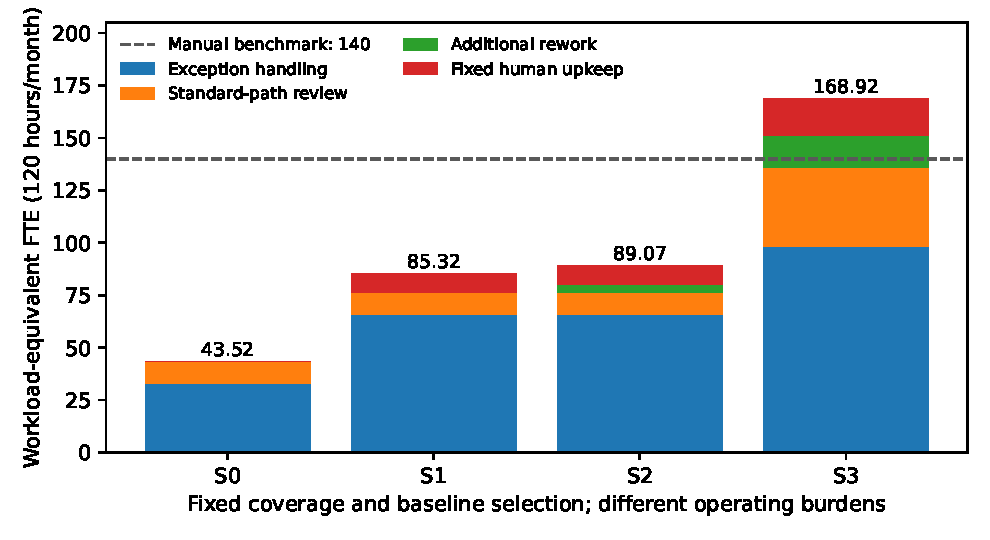
\includegraphics[width=0.88\linewidth]{figures/fig_components.pdf}
\caption{\textbf{The same coverage can release or consume human capacity.} Synthetic totals
decompose into exception handling, ordinary-path review, rework, and fixed upkeep. S0--S3 use the
same case volumes, exception fractions, and baseline selection; their post-deployment burdens differ.}
\label{fig:components}
\end{figure}

Equation~\eqref{eq:etastar} turns the same inputs into a fragility margin, reported in the last
column of Table~\ref{tab:partition}. Holding the S2 review, rework, and upkeep fixed, the exception
group could take 2.64 times its baseline effort in Security Architecture, 2.42 in Architecture, 1.81 in IT Production, 1.77 in Procurement and
in Compliance, and 1.60 in Tech Readiness before the saving disappears. For Legal, General Gate Support,
and Finance, whose residual holds two-thirds of
baseline labor, the margin is 1.20: a rise of about 20\% in exception effort erases the entire gain. The populations with the
largest exception share are the most exposed to post-deployment inflation.

These scenarios answer a conditional question: how much human work would the process require
at the specified operating burdens? They are not a probability distribution over future outcomes.
The notable result is not the most optimistic number but the failure of coverage to identify which
side of the frontier the process occupies. In an enterprise evaluation, the component quantities are
estimated prospectively and the forecast is tested on subsequent total hours.

\subsection{Same platform, different route economics}
\label{sec:routes}

The DGF routes differ in volume as much as in content. Integrations of inherited systems are rare and
heterogeneous; internal builds are frequent and more alike. Table~\ref{tab:routes} takes one
specialist team of 20 FTE with 100 monthly review visits and splits them into five Integrate visits
and 95 Build visits, each with $h_0=24$ hours. Both routes use
the same platform, 2.4 review hours and 0.5 rework hours per visit, and each carries 60 shareable plus
6 local upkeep hours per month: the playbooks, routing rules, and agent evaluations of
Section~\ref{sec:cases-parameters}. The Integrate route escalates 60\% of its visits, with $\kappa=1.4$ and
unchanged exception effort; the Build route escalates 14\%, with $\kappa=2$, and assistance
lowers exception effort by a fifth. A visit is a review work package, not a whole integration program. Both
partitions are coherent: $q\kappa=0.84$ for Integrate and 0.28 for Build, and Integrate's baseline
standard cases still cost 9.6 hours. The assumptions are synthetic, not measurements of the
framework's cases.

\begin{table}[!htb]
\centering\small
\caption{Route-specific illustration for one specialist team. Fixed upkeep is the same number of hours on both routes,
but its burden per visit differs.}
\label{tab:routes}
\begin{tabular}{@{}l r r r r r r r r@{}}
\toprule
Route & Visits & $q$ & $\kappa$ & $\phi$ & $\eta$ & Upkeep h/visit & $b_A$ & $\rho$\\
\midrule
\rowsinput{generated/table_routes_rows}
\bottomrule
\end{tabular}
\end{table}

\begin{figure}[!htb]
\centering
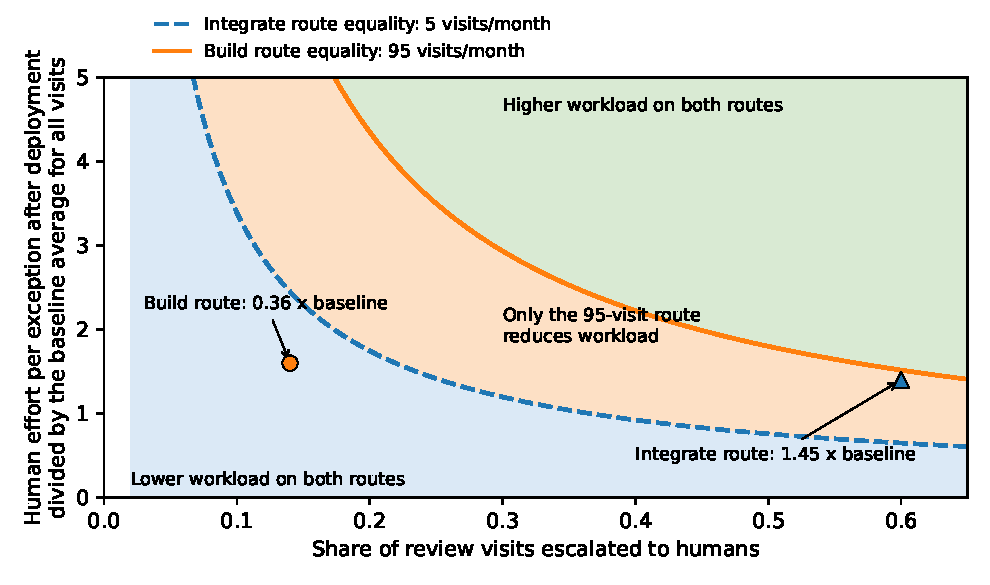
\includegraphics[width=0.84\linewidth]{figures/fig_frontiers.pdf}
\caption{\textbf{One platform, two workload frontiers.} Each route has 24 baseline hours per visit,
review at 10\% of that mean, 30 minutes of rework per visit, 60 shareable plus 6 local monthly upkeep
hours, and no separate baseline upkeep. The Integrate route has five visits per month; the Build route
has 95. Above a route's curve, its human workload exceeds its baseline. Markers show the two synthetic routes of Table~\ref{tab:routes}; volumes count review visits, not programs.}
\label{fig:frontier}
\end{figure}

The ratios are 1.451 and 0.360: opposite workload outcomes on the same platform
(Figure~\ref{fig:frontier}). The Integrate route combines concentrated residual labor with 13.2 upkeep
hours per visit, versus 0.69 on the Build route. Holding Integrate's other settings fixed but increasing
its volume to 95 visits lowers its ratio to 0.930: scale alone crosses its frontier. Sharing the sixty
common hours across 1,000 customers lowers it to 0.951 (Table~\ref{tab:provision}). A deployment that
would be a saving at scale is a loss at five visits a month.

The pooled ratio of 0.41 hides this: 8.29 residual FTE against 20. An enterprise reading only the
aggregate would miss that one route consumes more specialist time than before. These route curves and
points replace any presumption that one platform has one economic result.
